\documentclass[a4paper,12pt]{article}
\usepackage{graphicx}
\usepackage{cmap}
\usepackage[T2A]{fontenc}
\usepackage[utf8]{inputenc}
\usepackage{indentfirst}

%%\renewcommand{\footrulewidth}{ .0em }
\usepackage[english,russian]{babel}
\usepackage{multirow} % Слияние строк в таблице
\newcommand
{\un}[1]
{\ensuremath{\text{#1}}}



\begin{document}

\begin{titlepage}
	\begin{center}
		\large 	Московский физико-технический университет \\
		Физтех-школа радиотехники и компьютерных технологий\\
		\vspace{0.2cm}
		
		\vspace{4.5cm}
		Лабораторная работа № 3.2.2 \\ \vspace{0.2cm}
		\LARGE \textbf{Резонанс напряжений в электрическом контуре}
	\end{center}
	\vspace{2.3cm} \large
	
	\begin{center}
		Работу выполнил: \\
		Орловский Антон \\
		Б01-909

		
	\end{center}
	
	\begin{center} \vspace{60mm}
		г. Долгопрудный \\
		 2020 год
	\end{center}
\end{titlepage}




\paragraph*{Цель работы:} изучение последовательной цепи перемнного тока, наблюдение резонанса напряжений.
\paragraph*{Оборудование:} регулировочный автотрансформатор, катушка иднуктивности с выдвижным сердечником, магазин емкостей, реостат, резистор, амперметр, три вольтметра, ваттметр, осциллограм, универсальный мост.



\section{Теоретическое введение}

В теории переменных токов напряжения и токи принято выражать комплексными величинами. Модуль комплексной величины равен при этом амплитудному значению напряжения, а фаза - сдвигу фаз, измеренному по отношению к какому-либо одному напряжению или току, принятому в качестве опорного. Параметры основных элементов цепи задаются их импедансами, т.е тоже некоторыми комплексными числами.
\newline
Комплексную величину Z будет называть импедансом, комплексным сопротивлением последовательного контура:

\begin{equation}\label{}
Z = R + i(\omega L - \frac{1}{\omega C})
\end{equation}

\begin{figure}[h]
	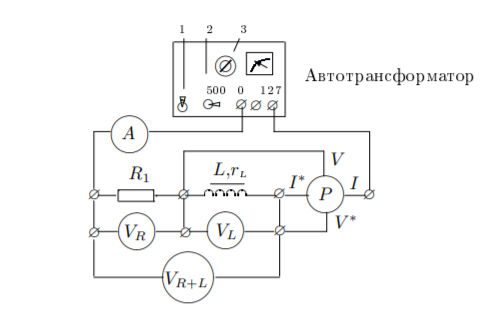
\includegraphics[width= 10cm]{Pic1.png}
	\caption{Схема установки для изучени закона Ома в цепи переменного тока}
	\label{Pic1}
\end{figure}

Электрическая цепь Рис.1 состоит из резистора $R$ и катушки индуктивности $L$ с импедансом $Z_L = r_L + i{\Omega}L$, последовательно подключенных к внешнему источнику, ЭДС которого меняется по синусоидальному закону с частотой $\Omega$.

Обозначим через $U_R$ нарряжение на резисторе, чрез $U_L$ напряжение на катушке, через $U_{R+L}$ напряжение на катушке и резисторе. Для этих напряжений справедливы комплексные соотношения.
\newline
Минуя их описание, а так же переход к модулям и фазам токов и напряжений, отметим, что измеряя с помощью трех вольметров значения $U_R$, $U_L$ и $U_{R+L}$ и зная сопротивление резистора, нетрудно вычислить силу точка в цепи, активное сопротивление катушки $r_L$, ее индуктивность $L$, мощность $P_L$, выделяемую на катушке и сдвиг фаз между током и напряжением на катушке.

\begin{equation}\label{}
U_R = {I}{R}
\end{equation}

\begin{equation}\label{r_l sq}
U_L = {I}{\sqrt{{r_L}^2 + ({\Omega}{L})^2}} 
\end{equation}

\begin{equation}\label{}
U_{L+R} = {I}{\sqrt{ (r_L + R)^2 + ({\Omega}{L})^2}} 
\end{equation}

Далее приведён итог расчета мощности переменного тока, выделяемой в катушке, через мнговенное значение мощности и интегрированием по всему периоду. 
\begin{equation}\label{}
P_L = U_L\cdot I\cdot cos(\psi) = I^2\cdot r_L
\end{equation}

Средняя мощность, выделяющаяся в катушке самоиндукции, определяется действительной частью ее импеданса.

Активное сопротивление катушки $r_L$, можно определить, если вклю-
чить её в последовательный колебательный контур с известными параметрами — сопротивлением R и ёмкостью С (рис. 2). В контуре, настроенном в резонанс на частоту $\Omega$ внешнего источника ( собственная частота контура и внешняя совпадают $\omega_0$ $=$ $\Omega$), реактивные сопротивления индуктивности и емкости одинаковы:

\begin{equation}\label{}
\omega_0 \cdot L = \frac{1}{\omega_0\cdot C}
\end{equation}

Определив каким-либо экспериментальным способом добротность Q этого контура, можно рассчитать полное сопротивление контура $R_{sum}$ в резонансе, поскольку:

\begin{equation}\label{}
Q = \frac{\omega_0 L}{R_{sum}} = \frac{1}{\omega_0 C R_{sum}}
\end{equation}

Резонансное сопротивление контура $R_{sum}$ включает в себя известное сопротивление резистора R и активное сопротивление катушки $r_L$

\begin{equation}\label{}
R_{sum} = R + r_L
\end{equation}

\begin{figure}[h]
	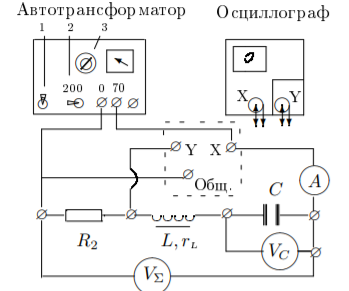
\includegraphics[width= 7cm]{Pic2.png}
	\caption{Схема установки для наблюдения резонанса напряжений}
	\label{Pic2}
\end{figure}





\section{Экспериментальная установка}
Схема установки для исследования
закона Ома в цепи переменного тока представлена на рис. 1. Цепь, состоящая из резистора $R \approx 100 Ом$ и катушки $L$ с выдвижным сердечником, подключена к автотрансформатору, выходное напряжение которого можно менять от 0 до 127 В. Напряжения на каждом из элементов
и суммарное напряжение цепи измеряются тремя вольтметрами: $V_R$, $V_L$ и $V_{L+R}$. Амперметр $А$ измеряет ток в цепи, а ваттметр $Р$ — мощность,
выделяющуюся на катушке

Схема установки для изучения резонанса напряжений изображена
на рис. 2. Последовательно соединены резистор $R \approx 5 Ом$, катушка $L$ и
магазин емкостей $С$. Амперметр $А$ измеряет ток в цепи, вольтметр $V_C$ —
напряжение на ёмкости, вольтметр $V_{\sum}$ — суммарное напряжение на кон-
туре. Резонанс можно зафиксировать с помощью осциллографа, если
подать на вход $X$ напряжение с контура, а на вход $Y$ — напряжение с
резистора $R_2$, пропорциональное току в цепи. В общем случае на экране
виден эллипс. При резонансе эллипс вырождается в прямую линию.

Резонансные напряжения на контуре $U_{\sum, res}$  и на ёмкости $U_C$,
равны соответственно.

\begin{equation}\label{}
U_{\sum, res} = I_{res}\cdot R_{\sum}
\end{equation}

\begin{equation}\label{}
U_{C,res} = \frac{I_{res}}{\Omega \cdot C}
\end{equation}

Сравнивая формулы (6), (7) и (8), получаем, что:


\begin{equation}\label{}
Q = \frac{U_{C, res}}{U_{\sum, res}}
\end{equation}

Формула (8) показывает, что добротность контура может быть найдена по измеренным значениям напряжений на контуре и на конденсаторе при резонансе. Зная добротность контура и ёмкость С, можно рассчитать $R_{\sum}$ по формуле (6), а затем определить $r_L$


\section{Ход работы}
\subsection{Закон Ома в цепи переменного тока.}

1) Снимем показания с вольтеметров, амперметра и ваттметра, импользуя формулы (2) и (3) рассчитываем значения для $  r_{L}$ и $ L $.

\begin{equation}\label{}
r_L = \frac{P_L}{I^2}
\end{equation}

\begin{equation}\label{}
L = \frac{1}{\Omega}\cdot\sqrt{\left(\frac{U_L}{I}\right)^2 - r_L^2)}
\end{equation}

Тогда погрешности будут:

\begin{equation}\label{}
\sigma_{r_L} = r_L \cdot \sqrt{(\frac{\sigma_{P_L}}{P_L})^2 + 4\cdot(\frac{\sigma_I}{I})^2}
\end{equation}

\begin{equation}\label{}
\sigma_{L} = L \cdot \sqrt{(\frac{\sigma_{P_L}}{P_L})^2 + 4\cdot(\frac{\sigma_I}{I})^2}
\end{equation}

\newline
Занесем полученные значения в таблицу 1.

Произведем расчет для среднего положения сердечника:

$$
r_L = 9.2 \:\text{Om}, \:
L = 1.09\: \text{H}
$$

Тогда погрешности:

$$
\sigma{r_L} = 0,27\: Om, \:\sigma_{L} = 0.03\: H.
$$


\begin{table}[h!]
	\centering
	\caption{Результаты измерений}
	\begin{tabular}{|c|c|c|c|c|c|c|c|}
		\hline
		$x_{disp}$ см & I, А & $U_R$, В & $U_L$, В & $U_{L+R}$, В & $P_L$, В & $L$, H $ \\
		\hline
		0,5 & 0,825 & 73 & 77  & 115 & 11,25 & 2,40  \\
		 \hline
		 0,7 & 0,875 & 78,5 & 68 & 113 & 10 & 2,10 \\
		 \hline
		 0,9 & 0,925 & 82,5 & 63 & 112 & 9,5 & 1,87\\
		 \hline
		 1,1 & 0,95 & 85,5 & 58 & 111 & 9 & 1,69\\
		 \hline
		 1,3 & 0,975 & 88 & 54 & 110,5 & 8,75 & 1,58\\
		 \hline
		 1,5 & 1,0125 & 90 & 51 & 110 & 8,25 & 1,46\\
		 \hline
		 1,7 & 1,02 & 91 & 48,5 & 110 & 8 & 1,38\\
		 \hline
		 1,9 & 1,025 & 92 & 46 & 109 & 7,75 & 1,31\\
		 \hline
		 2,1 & 1,028 & 92,5 & 44 & 109 & 7,5 & 1,24 \\
		\hline
	\end{tabular}% 
\label{resT}% 
\end{table}% 

\begin{table}[h!]
	\centering
	\caption{Рассчет $ r_{L}$ и $ L $ по формулам (3) и (5) }
	\begin{tabular}{|c|c|c|c|c|c|c|c|}
		\hline
		 $ L $, H & $ r_{L}$, Om \\
		\hline
		  1,84 & 16,53  \\
		 \hline
		  1,53 &  13,06 \\
		 \hline
		 1,34 &  11,1 \\
		 \hline
		 1,2 &  9,97\\
		 \hline
		 \textbf {1,09} & \texbf {9,2}\\
		 \hline
		 0,99 & 8,05\\
		 \hline
		 0,94 &  7,69\\
		 \hline
		 0,89 & 7,38\\
		 \hline
	     0,84 & 7,1 \\
		\hline
	\end{tabular}% 
\label{resT}% 
\end{table}% 

\begin{figure}[h!]
	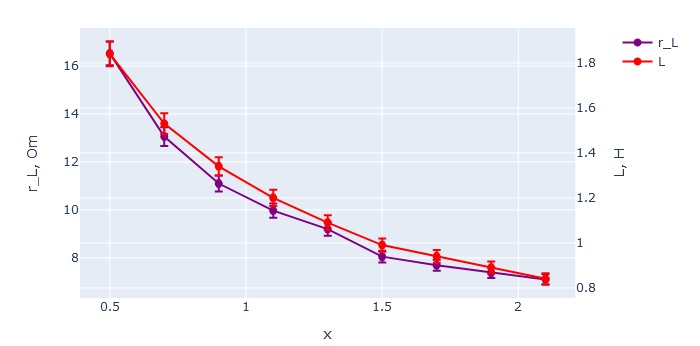
\includegraphics[width = 1.2\textwidth]{graph322 (1).jpg}
	\caption{Графики зависимостей}
	\label{Pic1}
\end{figure}


По результатам измерений составим таблицу и построим графики $ L(x) $ и $ r_{L}(x) $
\subsection{Векторная диаграма напряжений}

Для среднего положения сердечника построим векторную диаграму напряжений:

\begin{center}

\end{center}\

\begin{figure}[h]
	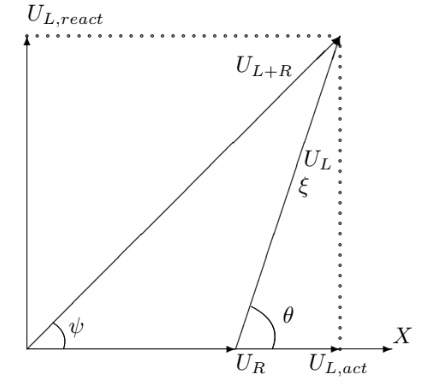
\includegraphics[width = 0.6\textwidth]{vect_diag.jpg}
	\caption{Векторная диаграмма}
	\label{Pic1}
\end{figure}


По теореме косинусов найдем угол $ {\psi} $ :


$$cos\psi = 0.88$$


Таким образом рассчитаем:

$$
U_{L,act} = {U_{L+R}}\cdot {cos\psi} - U_R = 9,24 V
$$

$$
U_{L,react} = U_{L+R}\cdot sin(\psi) = 52,47 \vspace{0.2cm} V
$$

Зная активное и реактивное сопротивление:

$$
L = \frac{U_{L,react}}{{I}{\Omega}} = 1,02 H
$$

$$
r_L = \frac{U_{L,act}}{I} = 9,48 Om
$$

Погрешности при данных измерениях составят:

\begin{equation}\label{}
\sigma_{r_L} = r_L \cdot \sqrt{(\frac{\sigma_{U_{L,act}}}{U_{L, act}})^2 + (\frac{\sigma_I}{I})^2}
\end{equation}

За погрешность вольметра берем половину цены деления.

\begin{equation}\label{}
\sigma_{L} = \sigma_{U_{L+R}} + \sigma_{U_R}
\end{equation}

По формулам (16), (17) получаем, что:

$$
    
$$


\subsection{Метод трех вольтметров} 
Вычислим значение $ P_{L} $ для резонансного положения сердечника 

С помощью векторной диаграммы выразим $P_L$ следующим образом:

$$
P_L = I\cdot U_L\cdot cos(\theta)
$$

,причем

$$
I = \frac{U_R}{R_1} \approx 0.89 \: A
$$
$$
U_L\cdot cos(\theta) = U_{L, act}
$$
Таким образом, получаем результат:
$$
P_{L} = 0.89 \: \text{A} \cdot 9.24 \: \text{V} \approx 8.22 \: \text{Watt}
$$

Рассчитанное значение мощности с помощью векторной диаграммы $P_{L,Vect} \approx 8.22$  Watt.
\newline
Показания ваттметра для среднего положения $P_{L}$ = 8.75 Watt. Нетрудно заметить, что полученные значения хорошо совпадают в пределах 5-ти процентов.

\subsection{Резонансное напряжение}
Рассчитаем активное сопротивление катушки $ r_{L}$ через значения резонансного тока и напряжения

$$
r_{L} = \frac{U_{\sum,res}}{I_{res}} - R_2 = 12.67 \: Om
$$


\begin{table}[h!]
	\centering
	\caption{Рассчет $ r_{L}$ через ток и напряжение }
	\begin{tabular}{|c|c|c|c|c|c|c|c|}
		\hline
		 I, А &  $U_{\sum}$, В & $ r_{L}$, Om \\
		\hline
		  3,35 & 62 &  12,67\\
		 \hline
	\end{tabular}% 
\label{resT}% 
\end{table}% 


\subsection{Расчеты через добротность}
Рассчитаем значения $ L $ и $ r_{L} $ через $ Q $ ( $ Q $ находим из формулы (8))

$$
L = \frac{1}{\omega_{0}^2\cdot C} \approx  12.8 \: H
$$

$$
r_{L} = \frac{{\omega_{0}}{L}}{Q} - R = 12,8 \: Om
$$


\subsection{Сведение результатов}
Сведем результаты измрения $ L $ и $ r_{L} $ для резонансного положения сердечника в таблицу 

\begin{table}[h!]
	\centering
	\caption{ Результаты измрения $ L $ и $ r_{L} $ }
	\begin{tabular}{|c|c|c|c|c|c|c|c|}
		\hline
		  &  Мультим.(при 0 Hz) & LCR & Вект.Диаг. &  $ f( I , $ U_{\sum} $) & $ f( $ Q $) $   \\
		\hline
		$ r_{L} $ , Om $ & 2.09  & 9.2 & 9.48 & 12.67 & 12.8\\
		\hline
		 L , H & - & 1.6 & 1.02 & - & 1.8 \\
		\hline
	\end{tabular}% 
\label{resT}% 
\end{table}% 


\section{Вывод}
Таким образом, мы экспериментально изучили резонанс напряжения в последовательной цепи переменного тока. Рассчитали сопротивление катушки и ее индуктивность тремя разными способами, соответственно посчитали погрешность.
\newline
Среднее значение полученных данных $ L  = (1,47 \pm0,04) \: H $ и $r_{L} = (11,04 \pm 0,27)$ Om для среднего положения сердечника (в том числе и при резонансе). 
\newline
Можем видеть, что погрешность составила примерно 3 процента. Основное расхождение в результатах при разных мпособах подсчета обуславливается потерями в проводах и погрешностями измерительных приборов.

\end{document}